\subsection{Early Fusion}

\begin{frame}[allowframebreaks]{Early Fusion: Key Ideas}
    \begin{itemize}
        \item \textbf{Stack frames as input channels to 2D CNN}
        \item Learns short-term motion patterns
        \item Limited receptive field along time
    \end{itemize}
\framebreak
    \begin{figure}
        \centering
        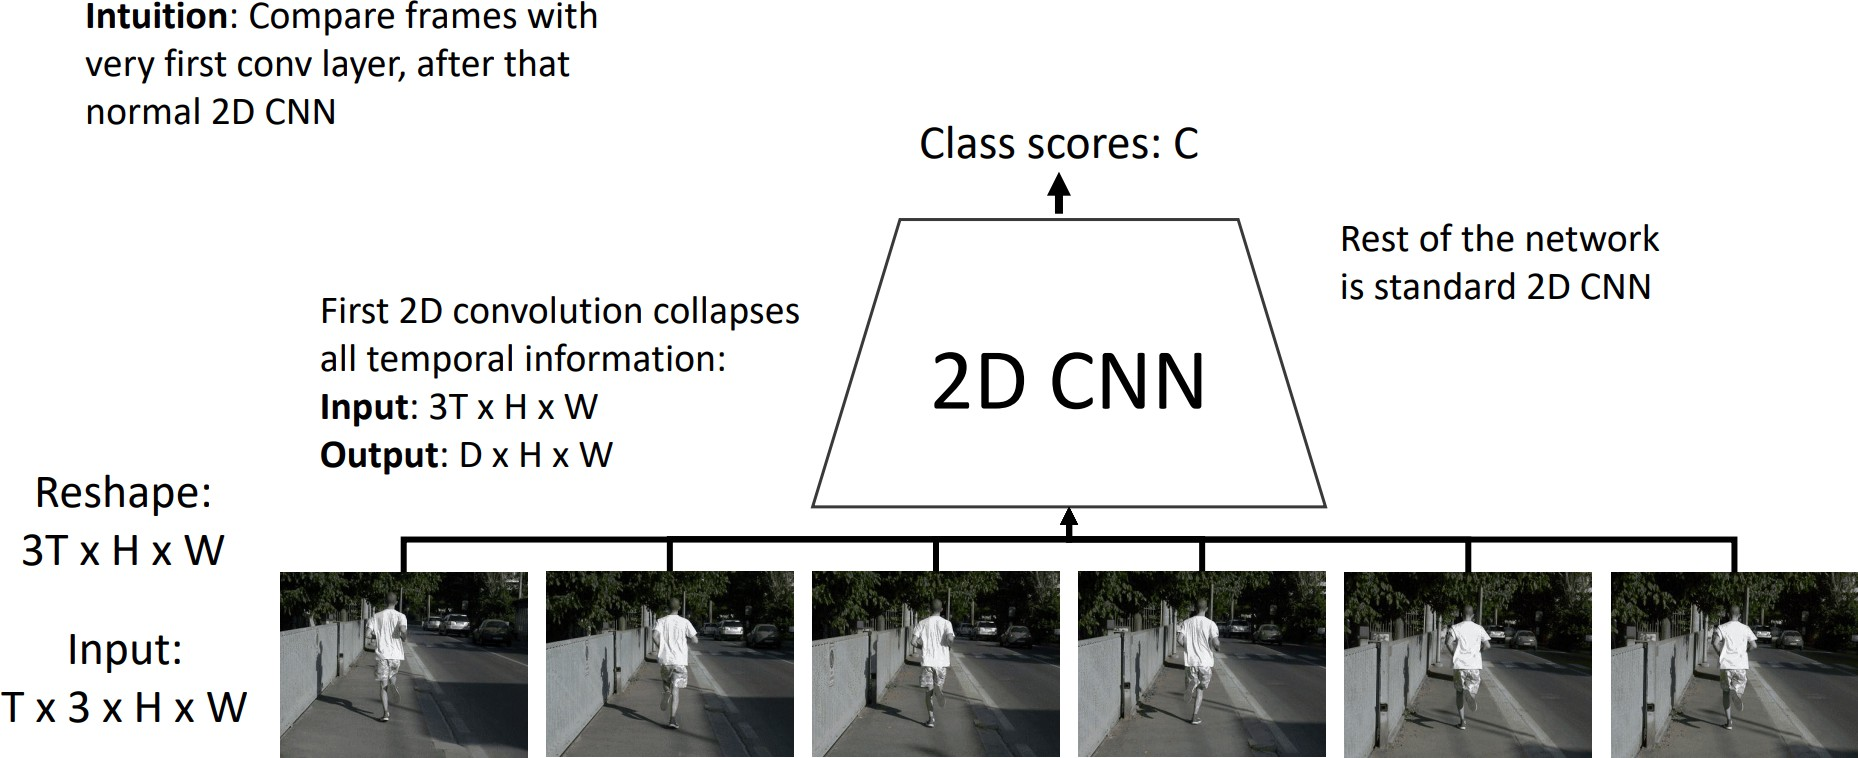
\includegraphics[width=1\textwidth,height=0.82\textheight,keepaspectratio]{images/video/slide_13_1_img.jpg}
        \caption*{\tiny [Source: UMich EECS 498 (2022), Lecture 24: Videos, slide 19]}
    \end{figure}
\framebreak
    \begin{figure}
        \centering
        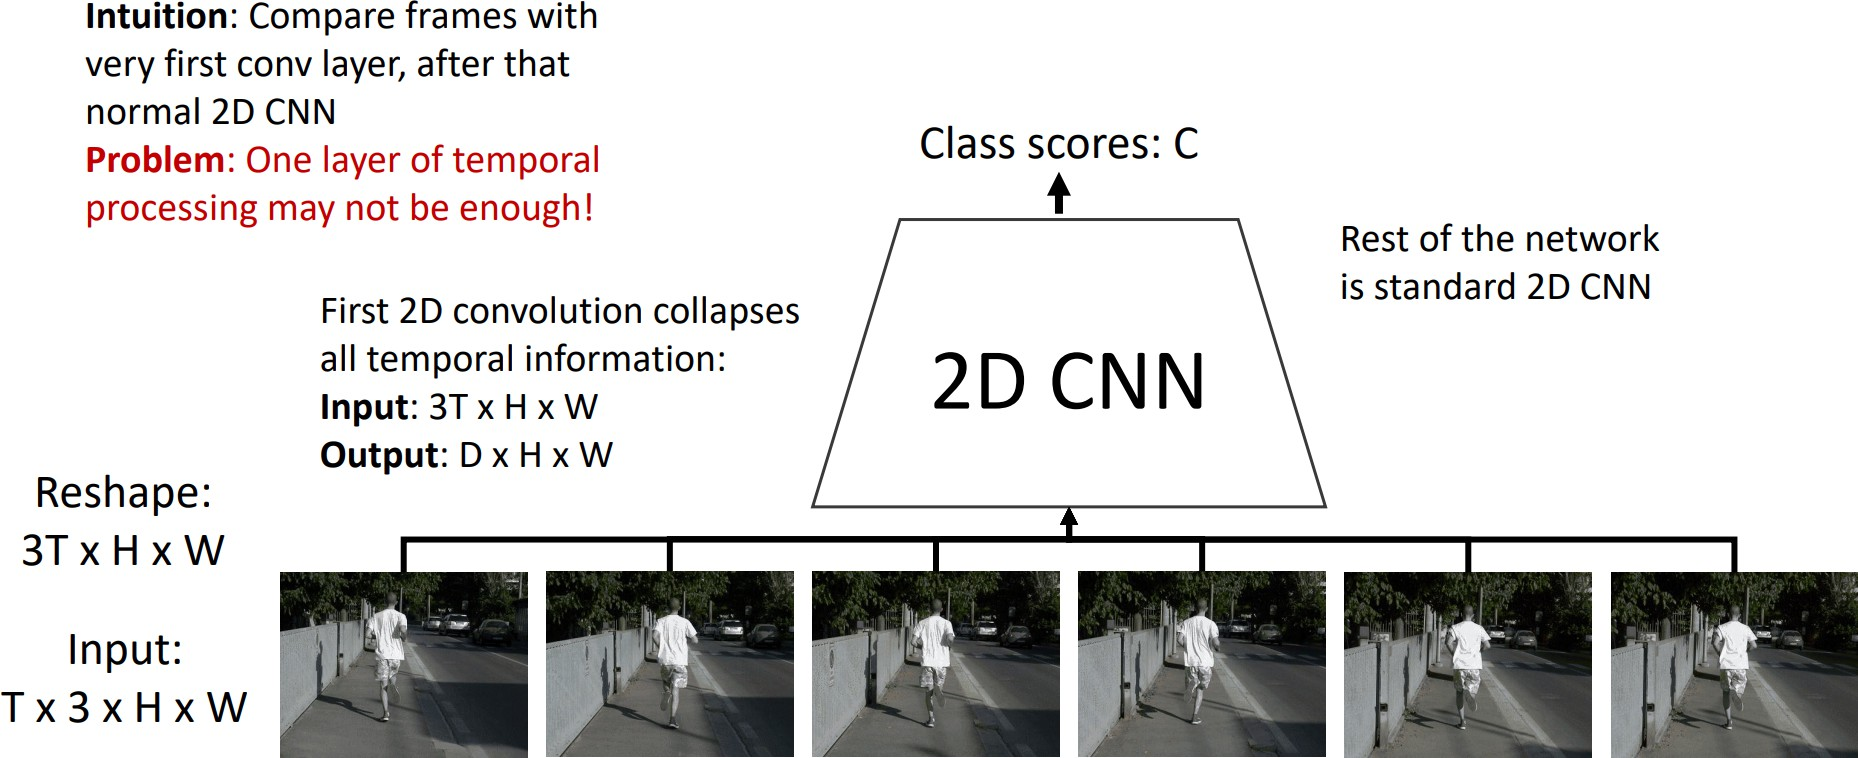
\includegraphics[width=1\textwidth,height=0.82\textheight,keepaspectratio]{images/video/slide_14_1_img.jpg}
        \caption*{\tiny [Source: UMich EECS 498 (2022), Lecture 24: Videos, slide 20]}
    \end{figure}
\end{frame}